\documentclass[10pt]{article}
\usepackage{graphicx}
\usepackage[margin=3cm]{geometry}
\usepackage[usenames,dvipsnames]{color}
\usepackage{array}
\usepackage[colorlinks=true, urlcolor=MidnightBlue]{hyperref}
\usepackage{fancyhdr}
\usepackage{fixltx2e} % \textsubscript
\usepackage{layout}

%%% Measurements %%%
% \topmargin=-0.3in
\oddsidemargin=0in
\evensidemargin=0in
\textwidth=6.5in
\marginparwidth=0.5in
% \headheight=0pt
\headsep=0pt
\textheight=670pt

%%% Table formatting %%%
\definecolor{lightgray}{gray}{0.8}
\newcolumntype{L}{>{\raggedleft}p{0.14\textwidth}}
\newcolumntype{R}{p{0.8\textwidth}}
\newcommand\VRule{\color{lightgray}\vrule width 0.5pt}

\title{JAMIE A. MACDONALD}
\author{\href{mailto:jamie.alban@gmail.com}{jamie.alban@gmail.com}\\(613) 583-7654\\2251 Fife Cres.\\Ottawa, ON}
\date{}

\renewcommand{\headrulewidth}{0pt} % no rule for header

\lfoot{\href{https://twitter.com/JamieMacdo}{@JamieMacdo}}
\cfoot{\href{https://github.com/jameh}{github.com/jameh}}
\rfoot{\href{https://ca.linkedin.com/in/jamiemacdo/}{ca.linkedin.com/in/jamiemacdo/}}

\begin{document}
%%% Center Name and email %%%
\begin{minipage}{0.2\textwidth}
\hspace{0em}
\end{minipage}
%%% Name and email %%%
\begin{minipage}{0.55\textwidth}
\vspace{-3em}
\maketitle
\end{minipage}
%%% Picture %%%
\begin{minipage}{0.25\textwidth}
\flushright{
    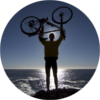
\includegraphics
    {jamie_alban_small.png}
}
\end{minipage}
\thispagestyle{fancy}
\vspace{-3em}
\section*{Objective}
I am looking for \textbf{fast-paced} summer employment in the field of \textbf{Software Development}. I have a strong \textbf{math and programming background} from my studies and hobbies, and I am excited by \textbf{elegant}, \textbf{innovative} solutions to human problems.
\vspace{-1em}
\section*{Education}
\begin{tabular}{L!{\VRule}R}
2010--2014&{\bf BSc Mathematics \& Engineering, Computing and Communication}\\
          &{Queen's University, Kingston Ontario}\\
\end{tabular}
\vspace{-1em}
\section*{Programming}
\textbf{Git} guru; \textbf{Python} web dev in Django, Flask; OOP; scripting; Abstract Syntax Tree parsing; Decorators; list comprehensions; Matplotlib, Scipy, Numpy; Sphinx; \textbf{Linux: bash, fish} scripting; \textbf{C} Makefiles, compiler flags, memory management; \textbf{Java} Generics, AWT, canvas; \textbf{C++} OOP; \textbf{Javascript}; Coffeescript; Nodejs, D3, jQuery; closures, modules, namespacing; \textbf{HTML}; Liquid, Jinja, Jade templates; \textbf{CSS}; SCSS, Stylus; Box model; \textbf{Octave, Matlab}; \textbf{LaTeX}; Algorithms, Data Structures

\vspace{-1em}
\section*{Mathematics}
\textbf{Probability}, Stochastic processes; \textbf{Information Theory}, Data Compression, \textbf{Communication Theory}, \textbf{Coding Theory}, Algebraic Structures; \textbf{Control Theory}, Differential equations, Linear time-varying systems; \textbf{Signals, Linear Systems}, \textbf{Transform Theory}, Sampling, Linear Algebra

\vspace{-1em}
\section*{Projects}
\begin{tabular}{L!{\VRule}R}
2013--2014&{\bf Channel-Optimized Vector Quantization of Correlated Images for Transmission over a Wireless Channel (Fourth Year Project/Thesis)}\\
          &{Implement a Lossy Joint Source-Channel Code which exploits the Correlation in two random sources (images)}\\
          &{(Information Theory, C programming, Python matplotlib, LaTeX writeup)}\\
2010&{\bf Child Soldier Cycle (Activism)}\\
    &{Biked 3000km from Ottawa to Newfoundland running an awareness campaign for child soldiering -- collected over 1500 red handprints as a petition to the media to provide better coverage of global Child Soldiering issues}\\
    &{Leadership, outreach, perseverance, organization}\\
\end{tabular}

\vspace{-1em}
\section*{Work Experience}
\begin{tabular}{L!{\VRule}R}
	Summer 2014&{\bf Software Programmer -- IBM Watson Visualization Engine}\\
			  &{Maintain charting/vis engine (Java); frontend JS demo app, evaluate API; D3js, jQuery; agile development; Java AWT, canvas; GeoJSON}\\
			  &{Collaborate with an international team; build strong communication skills}\\
\end{tabular}

\vspace{-1em}
\section*{Activities}
\textbf{Open Source contributions}: Openbox (C), Nitrogen (C++ GTK)\\
\textbf{Clubs}: Queen's Hack Nights\\
\textbf{Recreation}: Yoga, Rockclimbing, Biking, Longboarding\\

\end{document}
